\documentclass[11pt,letterpaper]{article}
\usepackage[left=1in,right=1in,top=1in,bottom=1in]{geometry}
\usepackage{amsmath,amsthm,amsfonts,amssymb,amscd}
\usepackage{bbm}
\usepackage{mathtools}
\usepackage{enumerate}
\usepackage{fancyhdr}
\usepackage{mathrsfs}
\usepackage{xcolor}
\usepackage{graphicx}
\usepackage{listings}
\usepackage{hyperref}
\usepackage{titlesec}
\usepackage{comment}
\usepackage{float}
\usepackage{url}

\hypersetup{%
  colorlinks=true,
  linkcolor=blue,
  citecolor=blue,
  urlcolor=blue,
  linkbordercolor={0 0 1}
}

\setlength{\parindent}{0.0in}
\setlength{\parskip}{0.1in}

\newcommand{\de}{\mathrm{d}}
\newcommand{\pe}{\partial}

\newcommand{\dsp}{\displaystyle}

\newcommand{\norm}[1]{\left\Vert #1 \right\Vert}
\newcommand{\mean}[1]{\left\langle #1 \right\rangle}

\newcommand{\ve}[1]{\boldsymbol{#1}}

\newcommand{\thus}{\Rightarrow \quad }
\newcommand{\fff}{\iff\quad}

\newcommand{\re}{\text{Re}}
\newcommand{\im}{\text{Im}}

\newcommand{\APE}{\text{APE}}
\newcommand{\KE}{\text{KE}}

\newcommand{\hot}{\text{h.o.t.}}
\newcommand{\inner}[2]{\left\langle #1,#2\right\rangle}

\newcommand{\ssp}{\left.\qquad\right.}

\newcommand{\var}{\text{var}}
\newcommand{\cov}{\text{cov}}

\newtheorem{theorem}{Theorem}[section]
\newtheorem{proposition}[theorem]{Proposition}
\newtheorem{lemma}[theorem]{Lemma}
\newtheorem{corollary}[theorem]{Corollary}
\newtheorem{remark}[theorem]{Remark}

\renewcommand\thesection{\arabic{section}}
\renewcommand\thesubsection{(\arabic{section}.\alph{subsection})}
\titleformat{\subsection}[runin]
        {\normalfont\bfseries}
        {(\arabic{section}.\alph{subsection})}% the label and number
        {0.5em}% space between label/number and subsection title
        {}% formatting commands applied just to subsection title
        []% punctuation or other commands following subsection title

\author{Ryan Shijie Du}
\date{\today}
\title{An Exploration of Semi-Lagrangian Methods for Advection
\\\vspace{0.3cm} \small Final Project for the Course: Computational Methods For Classical PDEs In The Physical Sciences}

\begin{document}

\newcommand{\sml}{\text{Semi-Lagrangian}}
\maketitle
\begin{abstract}
We explore using Semi-Lagrangian numerical methods to solve linear and nonlinear advection problem. The main benefit of \sml\ methods is that they are stable for large timestep. In particular it is stable for timestep size where the Courant–Friedrichs–Lewy (CFL) number defined in the traditional finite difference sense is larger than one. But for a \sml\;scheme to be accurate, we need to solve for the departure points and then interpolate the advected field onto the departure points, both to high accuracy. We explore several \sml\;schemes and reach fourth order space-time accuracy for linear advection where the advection velocity is known a priori. And for nonlinear advection, where the velocity is obtained from the advected field, we have third order. We also explore spectral interpolation and reach the same order of accuracy but without the need for spacial resolution refinement. 
\end{abstract}

\section{Introduction}
We want to solve the linear advection of a passive tracer, with the Partial Differential Equation (PDE):
\begin{align}
    \frac{\DD}{\DD t}c(\ve X(t),t) = \frac{\pe}{\pe t}c(\ve x,t)+\ve u(\ve x,t)\cdot\nabla c(\ve x,t) = 0\label{eq:linear_adv}
\end{align}
where $c$ is the concentration of the passive tracer of interests, $\ve X(t)$ is the Lagrangian trajectories of a fluid parcel (capital $\ve X$ denotes a marker for a particular fluid parcel), and $\ve u$ is the velocity is the underlying flow. We have the relation between $\ve X(t)$ and $\ve u$ is the ODE
\begin{align}
\frac{\de}{\de t}\ve X(t) = \ve u(\ve X(t),t).\label{eq:x_ODE}
\end{align}
\eqref{eq:linear_adv} says that for such a passive tracer without diffusion, the concentration $c$ is constant along the Lagrangian trajectory (i.e.: along $\ve X(t)$). 

From this fact, one might design a Lagrangian approach of solving \eqref{eq:linear_adv}, where we solve the ODE \eqref{eq:x_ODE} for a set of particles in time. Then the advection field $c$ at final time $T$ can be obtained from the knowing the final position of the particles since 
$$c(\ve X(0),0) = c(\ve X(T),T).$$
However, this approach degrades in accuracy in time since the initial will-spaced particles might evolve to irregular shapes and leaving big gaps where no information about $c$ is available. This problem is especially dire for compressible flows. 

\sml\;combines the Eulerian approach and the Lagrangian approach. In a nutshell, at each timestep we know $c$ at time $t$ on a regular \textit{Eulerian} grid $\ve x_i$ and we want to we calculate the information about $c$ at $t+\Delta t$ on the same regular \textit{Eulerian} grid. To do this, we use
$$c(\ve X_i,t+\Delta t) = c(\hat{\ve X}_i,t)$$
where $\hat{\ve X}_i$ is the departure point for the fluid parcel marked at $\ve X_i$ such that a \textit{Lagrangian} fluid trajectory goes through $\hat{\ve x}_i$ (resp. ${\ve x}_i$) at time $t$ (resp. $t+\Delta t$). The Lagrangian treatment of advection in each timestep allows for bigger time steps to be taken, and we still maintain the grid structure in Eulerian space. 

In general $\hat{\ve x}_i$ will not be on a grid point, therefore we need to interpolate to obtain an estimate. And except in trivial flows, we do not know the departure point $\hat{\ve x}_i$ exactly, and we need to numerically solve for an approximation. The main question to answer for \sml\;numerical method is how do we calculate the departure points $\hat{\ve{x}}_i$ and do the interpolation, and what are their properties. 
For the rest of the report we will explore several time integrating and space interpolation schemes of various order. We will use them to solve the linear advection problem \eqref{eq:linear_adv}, but also nonlinear advection problem like the 2D inviscid and incompressible Navier-Stokes equation \eqref{eq:2d_Nav}. The report will be organized as such: in Section \ref{sec:interp1D} we will test many interpolation schemes by using them to solve the 1D linear advection scheme with constant velocity. Section \ref{sec:linear_adv} contains the test of \sml\;Method on 2D linear advection problem (with constant and variable velocity field). !!!

\section{Interpolation Schemes, Tested in 1D Constant Advection}\label{sec:interp1D}
We first investigate the property of some interpolation scheme when used in Semi-Lagrangian methods. We solve 1D constant velocity advection problem: 
\begin{align*}
        \frac{\DD}{\DD t}c(x(t),t) = \frac{\pe}{\pe t}c(x,t)+ u \frac{\pe}{\pe x}c(x,t) = 0.
\end{align*}
This is because this problem is enough to show the properties of various interpolation schemes, and it is easy to visualize so that we can determine the nature of the error produced. Variable velocity case would not help with our investigation, since timestep error would pollute the interpolation error. %And it is harder to justify \eqref{eq:linear_adv} in 1D when velocity is non-constant and thus compressible (but possible, see \cite[(1-3)]{diamantakis}). 

We set the domain to be $[0,1)$ periodic, and solve for $t\in [0,1]$. $u = 1$ constant so that at $T = 1$, the tracer should be advection around the domain to its original position. This provide us with a test of accuracy of the solution. Since $u$ is constant, we know the departure points a priori thus interpolation is the only source of errors. There is no error in time, we fix the timestep constant as 7 (this is an odd number, and $Nx$ is always even, to ensure that we are not landing on a grid point). To investigate the order of convergence for the interpolation method, we vary the spacial resolution ($Nx = 8:1024$). Note that our CFL number is larger than one and reaching about 150 when the spatial resolution is the most dense. This corroborate the fact that the \sml\;method is unconditionally stable. We solve the problem with a power of trigonometric function initial condition:
\begin{align*}
    c(x,0) &= [\sin(\pi x)]^p \hspace{1cm}\text{with }p = 40.
\end{align*}

We investigate a handful of interpolation methods implemented in MATLAB's \texttt{interp1} function as well as spectral interpolation method based on Flatiron Institute Nonuniform Fast Fourier Transform (FINUFFT) \cite{finufft_1,finufft_2}. Note that for MATLAB's \texttt{interp1} function, we feed it padded data where we extend the function on the left and right by five points using periodicity. For all query point, we mod it to make sure that it says within $[0,L)$. (We do not use Lagrange polynomial interpolation mostly since I could not find a good implementation in MATLAB available.\footnote{In my search, I saw claims that there is a reason why (quadratic and cubic) Lagrange polynomial is not implemented in MATLAB, and it is because it is a bad idea. But I could not figure out why it is a bad idea. I don't think it is because of the Runge's phenomenon since it is only application when the polynomial order is higher than 3.}) We start with \texttt{linear}, which is Lagrange linear interpolation. Fig. \ref{fig:1D_cons_linear_} shows the result: the left is comparison of the numerical solutions to the truth, and the right is the plot for order of convergence. We see that the error is mainly diffusive, and the order of the interpolation is second. For constant velocity, \sml\;method is equivalent to the upwind method when the CFL number is less then one. Therefore it is reassuring to see that the nature of the error is the same (diffusive).
\begin{figure}[H]
    \centering
    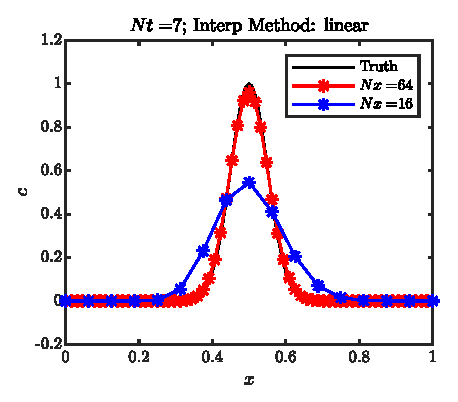
\includegraphics{figs/1D_cons_linear_sol}
    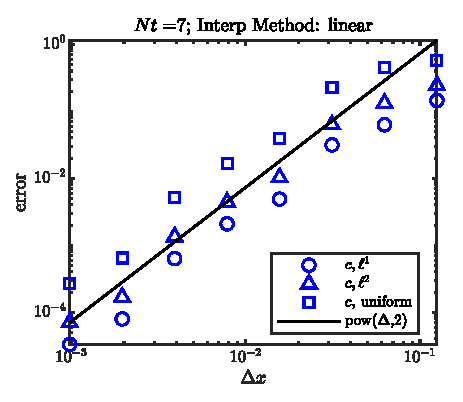
\includegraphics{figs/1D_cons_linear_convord}
    \caption{}\label{fig:1D_cons_linear_}
\end{figure}
Now we look at \texttt{cubic}, which is not cubic Lagrangian, but instead the cubic interpolation in \cite{keys_cubic_1981} and \texttt{spline}, cubic spline. Fig. \ref{fig:1D_cons_cubic_} and Fig. \ref{fig:1D_cons_spline_} shows the result for \texttt{cubic} and \texttt{spline} respectively. For both methods, the error is both diffusive and dispersive. The convergence order of \texttt{cubic} is third, this corroborate that this is not cubic Lagrangian, since it should be of fourth order. Cubic \texttt{spline} is of fourth order, as we expected.
\begin{figure}[H]
    \centering
    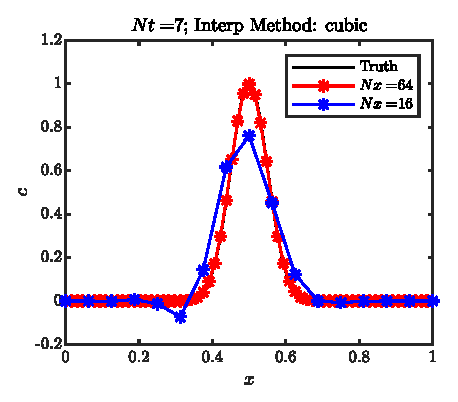
\includegraphics{figs/1D_cons_cubic_sol}
    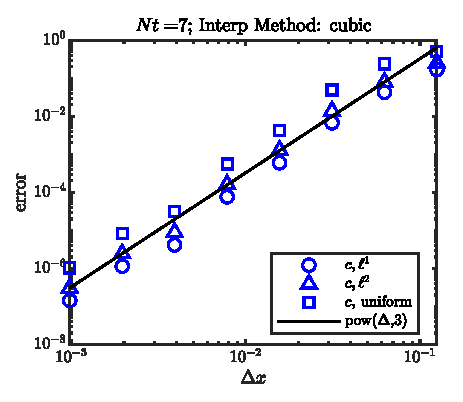
\includegraphics{figs/1D_cons_cubic_convord}
    \caption{}\label{fig:1D_cons_cubic_}
\end{figure}
\begin{figure}[H]
    \centering
    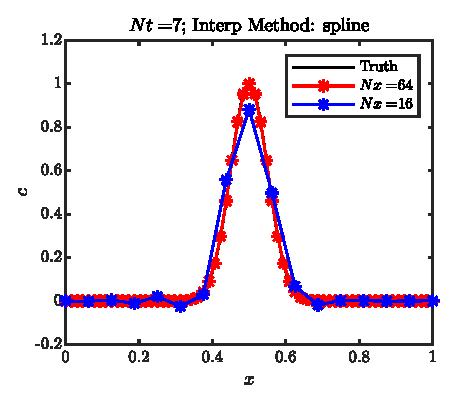
\includegraphics{figs/1D_cons_spline_sol}
    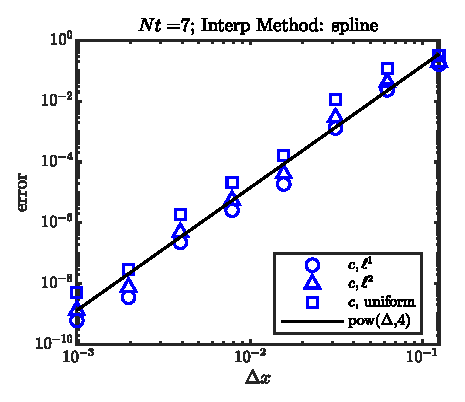
\includegraphics{figs/1D_cons_spline_convord}
    \caption{}\label{fig:1D_cons_spline_}
\end{figure}
Next, FINUFFT. Since our data is periodic and on a regular grid, we can calculate its Fourier representation using regular \texttt{fft}. Then to evaluate the Fourier series on an nonuniform mesh (for non-constant velocity case), we use FINUFFT type 2 \cite{finufft_1}. This means that to interpolate $N$ non-uniform points from $N$ uniform known data, the cost is $O(N\log N)$ instead of $O(N^2)$. In comparison, all other interpolation method presented here is of cost $O(N)$. Spectral interpolation is more expensive, but not prohibitively so. Fig. \ref{fig:1D_cons_finufft_} shows the result. We see that the interpolation using a coarse space grid is still accurate, though there is a small magnitude oscillation on the two side where the truth is constant. The dense space grid result is perfect. For this grid we have enough points to fully represent the initial conditions Fourier spectrum. Also note that the order of convergence is indeed spectral.
\begin{figure}[H]
    \centering
    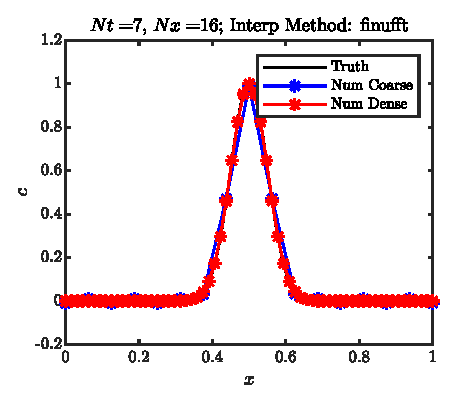
\includegraphics{figs/1D_cons_finufft_sol}
    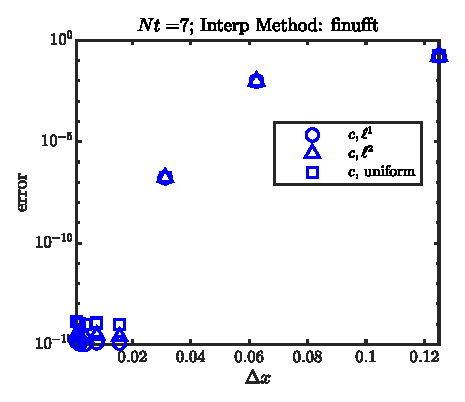
\includegraphics{figs/1D_cons_finufft_convord}
    \caption{}\label{fig:1D_cons_finufft_}
\end{figure}
Finally, we study \texttt{pchip} and \texttt{makima}. They are similar in that they are both piecewise polynomial of order the most three, and they are designed to prevent overshoot. Fig. \ref{fig:1D_cons_pchip_} (resp. Fig. \ref{fig:1D_cons_makima_}) shows the result for \texttt{pchip} (resp. \texttt{makima}). The error is diffusive, it is also dispersive since the peak is asymmetric. But there is no undershoot on the left of the peak compared to \texttt{cubic} and \texttt{spline} in Fig. \ref{fig:1D_cons_cubic_} and Fig. \ref{fig:1D_cons_spline_}. This is a good feature since a negative tracer concentration $c$ is nonphysical (cf. limiters). The order of convergence of these two methods is not the same as the above methods. The uniform norm convergence order is one less than the convergence order in other norms. This is probably due to the corrections at extrema. 
\begin{figure}[H]
    \centering
    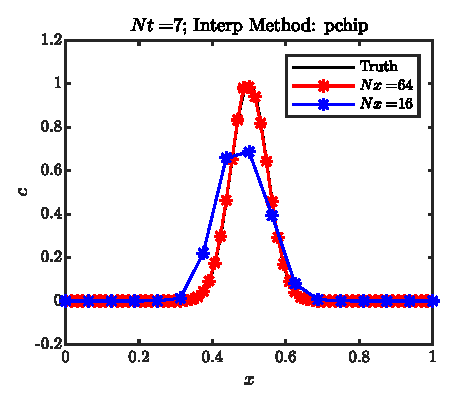
\includegraphics{figs/1D_cons_pchip_sol}
    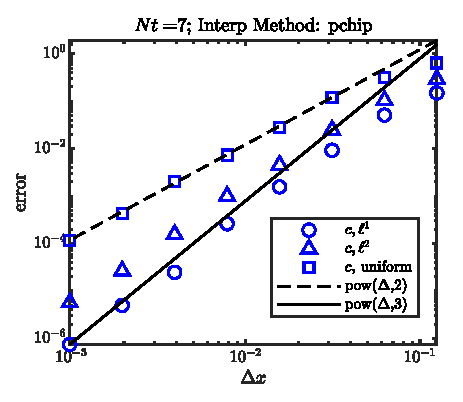
\includegraphics{figs/1D_cons_pchip_convord}
    \caption{}\label{fig:1D_cons_pchip_}
\end{figure}
\begin{figure}[H]
    \centering
    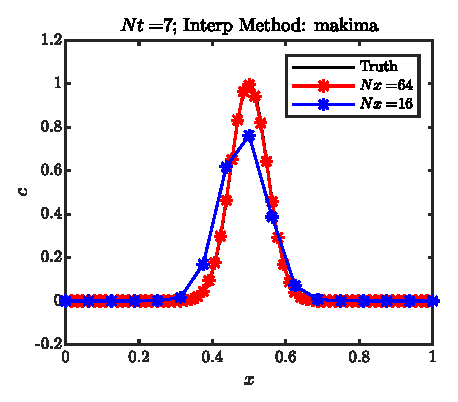
\includegraphics{figs/1D_cons_makima_sol}
    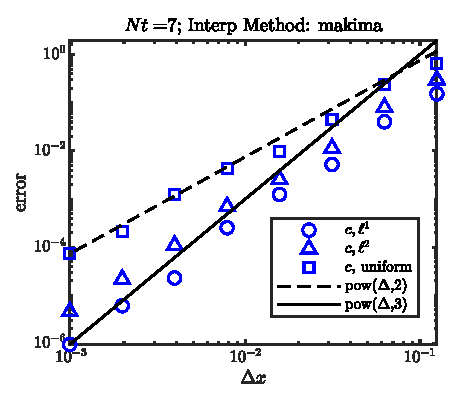
\includegraphics{figs/1D_cons_makima_convord}
    \caption{}\label{fig:1D_cons_makima_}
\end{figure}

The truth strength of \texttt{phip} and \texttt{makima} shows when we try to use this method to advect a step function, and that is what we will experiment on now. We set the initial condition to be a step function:
\begin{align*}
    c(x,0) &= \chi_{(1/4,1/2)}.
\end{align*}
We first show the result for \texttt{linear} in Fig. \ref{fig:1D_step_cons_linear_}. We see that the error is still diffusive, but the order of convergence is no longer one. This is because the convergence theory is based on Taylor series, which clearly does not apply for a step function.
\begin{figure}[H]
    \centering
    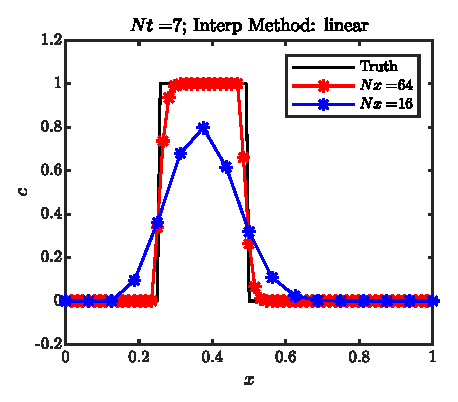
\includegraphics{figs/1D_step_cons_linear_sol}
    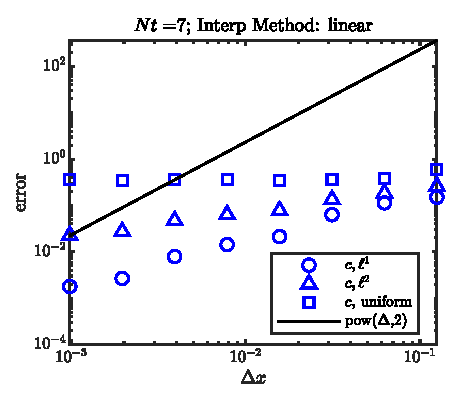
\includegraphics{figs/1D_step_cons_linear_convord}
    \caption{}\label{fig:1D_step_cons_linear_}
\end{figure}
The order of convergence result does not look too difference from the right plot of Fig. \ref{fig:1D_step_cons_linear_} for \texttt{cubic}, \texttt{spline}, \texttt{pchip}, and \texttt{makima}, thus we will not show them. But the qualitative nature of the error are vert different and it is worse looking at and analyzing. \texttt{cubic} and \texttt{spline} has large oscillation near the discontinuity accompanied with overshoot and undershoot, as shown in Fig. \ref{fig:1D_step_cons_cubic_sol}.
\begin{figure}[H]
    \centering
    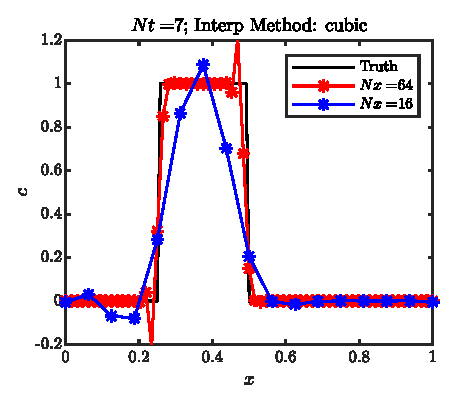
\includegraphics{figs/1D_step_cons_cubic_sol}
    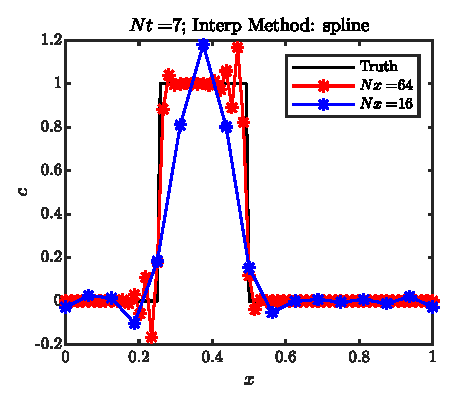
\includegraphics{figs/1D_step_cons_spline_sol}
    \caption{}\label{fig:1D_step_cons_cubic_sol}
\end{figure}
In comparison \texttt{pchip} and \texttt{makima} does not have such issue, as shown in Fig. \ref{fig:1D_step_cons_pchip_sol}. This suggests that these two interpolation scheme is good for solving problems with discontinuities, say from shock. 
\begin{figure}[H]
    \centering
    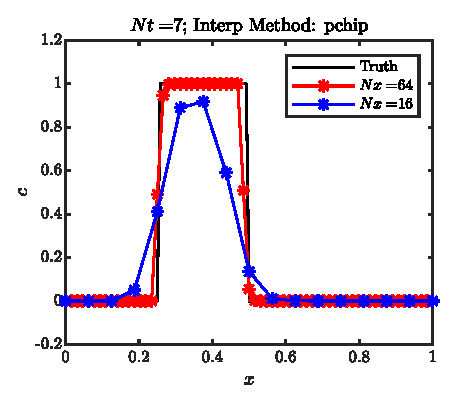
\includegraphics{figs/1D_step_cons_pchip_sol}
    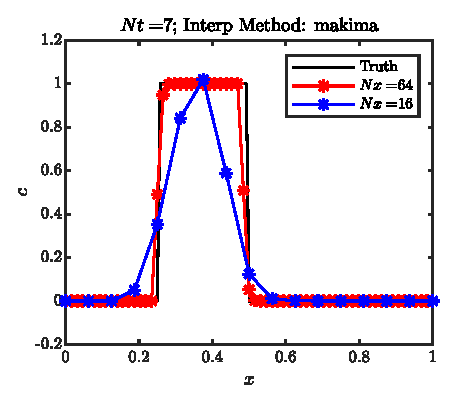
\includegraphics{figs/1D_step_cons_makima_sol}
    \caption{}\label{fig:1D_step_cons_pchip_sol}
\end{figure}
Finally, we show the result from FINUFFT in Fig. \ref{fig:1D_step_cons_finufft_sol}. There is oscillation at the smallest scale of the resolution. This is likely due to the fact that for a discontinuous function, the Fourier coefficient decays very slowly. This fact is also represented in the error graph, now in \texttt{loglog} form, we can see that the error only converges in first order. 
\begin{figure}[H]
    \centering
    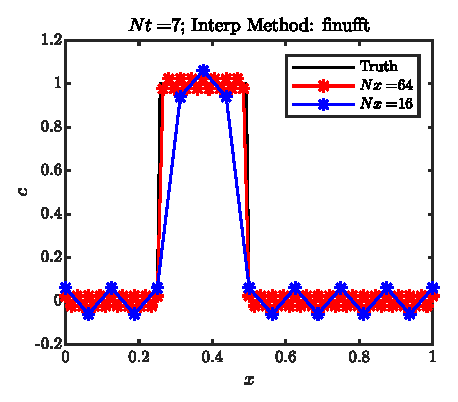
\includegraphics{figs/1D_step_cons_finufft_sol}
    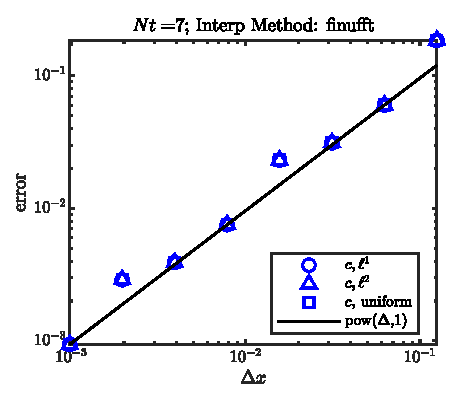
\includegraphics{figs/1D_step_cons_finufft_convord}
    \caption{}\label{fig:1D_step_cons_finufft_sol}
\end{figure}

Wrapping up this section, we have experimentally investigated the nature of the error and the order of convergence of various interpolation methods implemented in MATLAB's \texttt{interp1} function as well as a spectral interpolation method. We will use \texttt{linear}, \texttt{cubic}, \texttt{spline}, and FINUFFT for the future sections. We will not use \texttt{pchip} and \texttt{makima} since they are only significantly different when the solution is discontinuous, but all our future example will be continuous. Also, they will make the order of convergence study of the full \sml\;scheme more confusing. But they should be considered when we run into future problems when there is discontinues in the solutions. 


\section{Semi-Lagrangian Method for 2D Linear Advection}\label{sec:linear_adv}
We verify the lesson we learn from Section \ref{sec:interp1D} in 2D. We solve again the constant velocity advection problem with $[0,1)\times [0,1)$ with $\ve u = (1,1)$. We solve to $T = 2$ and compare the solution to the initial condition. We use a 2D trigonometric polynomial as initial condition:
\begin{align}
    c(x,y,0) &= [\sin(\pi x)\sin(\pi y)]^p \hspace{1cm}\text{with }p = 2.\label{eq:sinp2}
\end{align}
We use $Nt = 15$ and $Nx = Ny = 8:256$ (CLF number = $1.2:34$). We show the resultant convergence order estimate in Fig. \ref{fig:2D_const_adv_all_interp}. We see that the order of convergence for \texttt{linear}, \texttt{cubic}, and \texttt{spline} are the same with the result in Section \ref{sec:interp1D}. And FINUFFT is accurate for all spatial resolution since our initial condition only needs a few Fourier mode to be represented accurately. 
\begin{figure}[H]
    \centering
    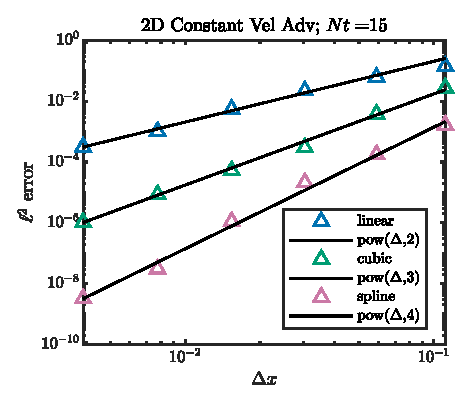
\includegraphics{figs/2D_const_adv_all_interp}
    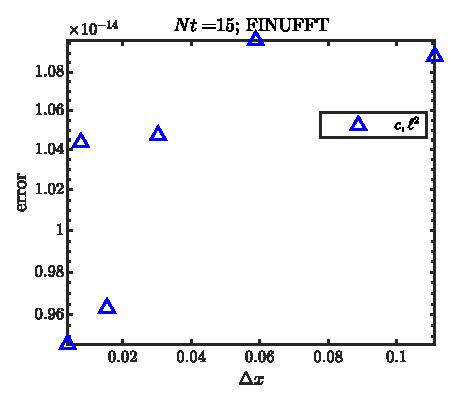
\includegraphics{figs/2D_const_adv_finufft}
    \caption{}\label{fig:2D_const_adv_all_interp}
\end{figure}

Now we are familiar with the interpolation step of \sml\;methods, we deal with the time integration step. We first focus on solving the linear advection problem where we assume the velocity $\ve u$ is known at all time on the spatial grid. In particular, for the timestep from $t^n$ to $t^{n+1/2}$, we know for all $x_i$ on the spatial grid:
\begin{align*}
    \ve u_i^{n} &= \ve u(\ve x_i,t^n);\\
    \ve u_i^{n+1/2} &= \ve u(\ve x_i,t^{+1/2});\\
    \ve u_i^{n+1} &= \ve u(\ve x_i,t^{n+1}).
\end{align*}
With these information, and the ``initial'' condition that $\ve X(t^{n+1}) = \ve x_i$ a grid point, we need to solve the ODE \eqref{eq:x_ODE} backward in time to obtain $\hat{\ve x}_i = \ve X(t^{n})$. The first method is to use a (backward) Euler step:
\begin{align*}
    \frac{\hat{\ve x}_i-\ve X(t^{n})}{\Delta t} = \frac{\ve X(t^{n+1})-\ve X(t^{n})}{\Delta t} = \ve u(\ve X(t^{n+1}),t^{n+1}) = \ve u(\ve x_i,t^{n+1}).
\end{align*}
The error in the departure point estimate $\hat{\ve x}^{(1)}_i$ is $\norm{\hat{\ve x}^{(1)}_i-\hat{\ve x}_i} = O(\Delta t^2)$ (cf. local truncation error for backward Euler). To match the time error, a second order linear interpolation of $c$ onto $\hat{\ve x}_i$ would suffice. Together the space-time local truncation error $O(\Delta t^2+\Delta x^2)$. Indeed, name the interpolated tracer to be $\overline{c}$, we have by triangular inequality
\begin{align*}
    \norm{\overline{c}(\hat{\ve x}^{(1)}_i,t^n)-c(\hat{\ve x}_i,t^n)} &\leq \norm{\overline{c}(\hat{\ve x}^{(1)}_i,t^n)-\overline{c}(\hat{\ve x}_i,t^n)}+\norm{\overline{c}(\hat{\ve x}_i,t^n)-c(\hat{\ve x}_i,t^n)}\\
    &\leq \text{Const}\cdot \norm{\hat{\ve x}^{(1)}_i-\hat{\ve x}_i}+O(\Delta t^2) = O(\Delta x^2+\Delta t^2).
\end{align*}
Now global error of this method is one less than the local truncation error, thus we have a first order space-time accurate method. 

We test the order of convergence on a sample problem. We use the inviscid Taylor vortex as our underlying velocity ($v_0 = 1, L = 2\pi$):
\begin{align}
    u &= v_0-\cos\left(\frac{2\pi(x-v_0t)}{L}\right)\sin\left(\frac{2\pi(y-v_0t)}{L}\right)\nonumber\\
    v &= v_0+\sin\left(\frac{2\pi(x-v_0t)}{L}\right)\cos\left(\frac{2\pi(y-v_0t)}{L}\right).\label{eq:taylor}
\end{align}
And the initial tracer distribution is the three Gaussian peaks:
\begin{align}
    c(x,y,0) =& \exp\left( -5\left((x-\pi)^2+(y-3\pi/4)^2\right) \right)+\exp\left( -5\left((x-\pi)^2+(y-5\pi/4)^2\right) \right)\nonumber\\
    &-\frac{1}{2}\exp\left( -\frac{5}{2}\left((x-5\pi/4)^2+(y-5\pi/4)^2\right) \right).\label{eq:3Gauss}
\end{align}
We solve the problem numerically till $T = 0.5$ and empirically estimate the error. We can also compare the solution to the ``truth'' solution obtained by using the Pseudospectral IF-RK4 method from HW3. The convergence order plots look the same and we will only show the empirical estimates. First, Fig. \ref{fig:c_init_IF} shows the initial distribution of the tracer and a ``truth'' solution from Pseudospectral IF-RK4:
\begin{figure}[H]
    \centering
    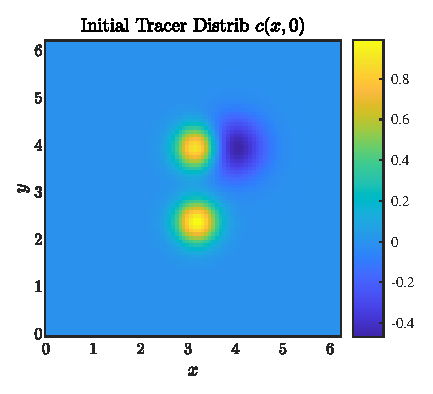
\includegraphics{figs/c_init_IF-RK4PS}
    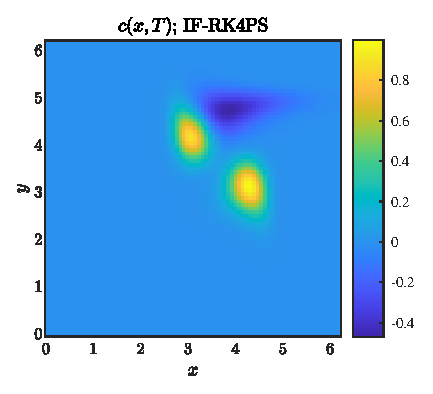
\includegraphics{figs/c_final_IF-RK4PS}
    \caption{}\label{fig:c_init_IF}
\end{figure}
Then Fig. \ref{fig:c_final_Euler} shows on the left the tracer concentration that is solved by Euler Method at the finest space-time resolution and on the right the order of convergence from the empirically estimated error. Here we use $Nx = Ny= [2^5:2^{10}]$ but large timestep such that the CFL number $v_0\Delta t/\Delta x = 1.5$. This means $Nt = 3:55$, not many timesteps! (Note that Taylor vortex is a special flow that if we use it to advect a tracer for too long, the tracer field will develop small scale features that is hard to solve, thus we have chosen the rather short time window. Read Section \ref{sec:adv_NS} see an example with a larger time window.)
\begin{figure}[H]
    \centering
    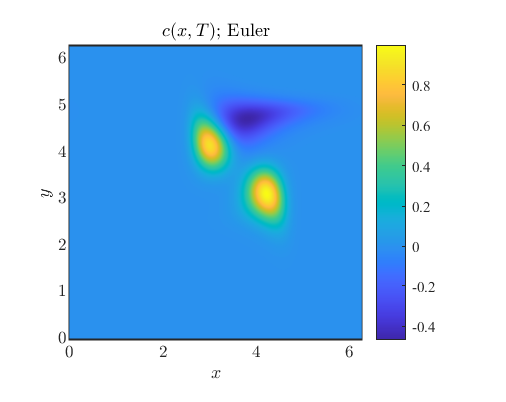
\includegraphics{figs/c_final_Euler}
    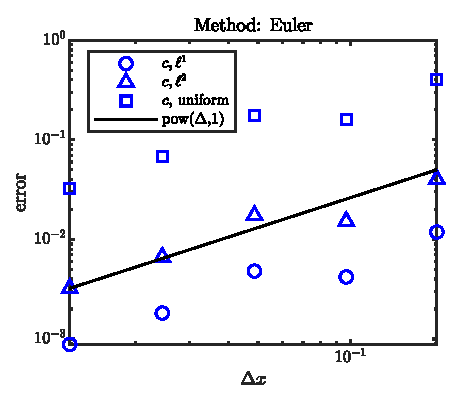
\includegraphics{figs/conv_order_Euler}
    \caption{}\label{fig:c_final_Euler}
\end{figure}

A higher order method for solving ODE is the trapezoidal method. To generalize it to \sml\ method, we need to estimate the velocity at the departure point at $t^n$: $\ve u(\hat{\ve x}_i,t^n)$. We write the trapezoidal rule for the ODE \eqref{eq:x_ODE}:
\begin{align*}
    &\ve X(t^{n+1})-\ve X(t^{n}) = \frac{\Delta t}{2}\left[\ve u(X(t^{n}),t^n)+\ve u(X(t^{n+1}),t^{n+1})\right]\\
    \fff &\ve x_i-\hat{\ve x}_i = \frac{\Delta t}{2}\left[\ve u(\hat{\ve x}_i,t^n)+\ve u(\ve x_i,t^{n+1})\right].
\end{align*}
We have in our hand for each $i$ a nonlinear equation, we can solve this via fix point:
\begin{align*}
    \hat{\ve x}_i^{(k+1)} = \ve x_i-\frac{\Delta t}{2}\left[\ve u(\hat{\ve x}_i^{(k)},t^n)+\ve u(\ve x_i,t^{n+1})\right]
\end{align*}
and we start the iteration by estimating $\hat{\ve x}_i^{(0)} = \hat{\ve x}_i$. As it turns out, to reach global second order accuracy and local third order accuracy, the highest that trapezoidal rule could reach, we only need to do one fixed point iterations and obtain $\hat{\ve x}_i^{(1)}$. Then we have the tracer field at time $t^{n+1}$ (remember that over-line means interpolated result)\footnote{This is just two fixed point iterations, but separating out the last evaluation from the fixed point iteration makes the concept of iteration number more consistent with the next MCD86 method.}
\begin{align*}
    &\hat{\ve x}_i^{(2)} = \ve x_i-\frac{\Delta t}{2}\left[\ve u(\hat{\ve x}_i^{(1)},t^n)+\ve u(\ve x_i,t^{n+1})\right]\\
    &c({\ve x}_i,t^{n+1}) = \overline{c}(\hat{\ve x}_i^{(2)},t^{n}).
\end{align*}
A similar bound using triangular inequality is also possible for this method and it shows that we need a third order interpolation for interpolating the tracer field, thus we use \texttt{cubic}. We also need to interpolate to get the velocity field at $\hat{\ve x}_i^{(1)}$, as it turns out we only need second accuracy for that, thus we use \texttt{linear}. It is important to use the cheapest interpolation scheme possible since interpolation is the main of \sml\ method. This fact is mentioned in \cite{staniforth1991}: 
\begin{quote}
    ``For step (i), the order of the interpolation is much less important. Theoretically, McDonald (1987) has shown that one should use an interpolation of order one less than for step (ii).''
\end{quote}
Here McDonald (1987) refers to \cite{mcdonald1987}. Note that there are many other global space-time second order method, for example ones based on mid-point rule. Some examples are given in \cite{mcdonald1999} and in there the author provide a general formula for second order accurate schemes. I am not sure what are the differences between all of them and I only investigate this trapezoidal method because I thought it is the most conceptually simplistic. Now we show result, Fig. \ref{fig:c_final_Trap} shows the final tracer field on the let and the order of convergence result on the right. We see that the tracer fields look the same with the ``truth'' and the order of convergence is as expect, second order.
\begin{figure}[H]
    \centering
    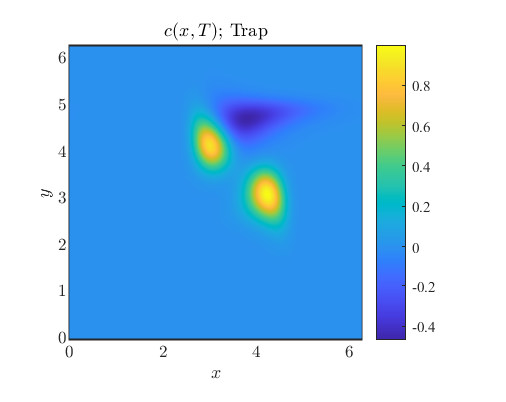
\includegraphics{figs/c_final_Trap}
    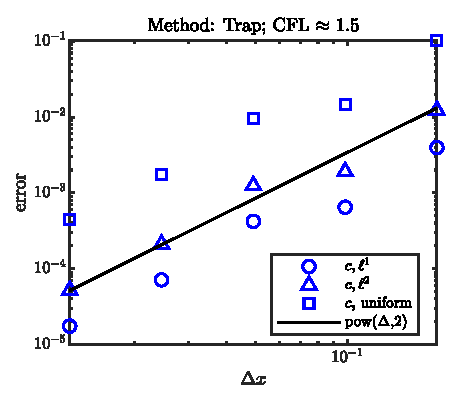
\includegraphics{figs/conv_order_Trap}
    \caption{}\label{fig:c_final_Trap}
\end{figure}

\cite{mcdonald1987} presents a global space-time third order accurate method. We first solve two nonlinear equations:
\begin{align*}
    &\ve X(t^{n+1})-\ve X(t^{n+1/2}) = \frac{\Delta t}{2}\left[\ve u(X(t^{n+1/2}),t^{n+1/2})\right];\\
    &\ve X(t^{n+1})-\ve X(t^{n}) = {\Delta t}\left[\ve u(X(t^{n}),t^{n})\right].
\end{align*}
It turns out we need to do two iterations, then we evaluate the midpoint rule and get:
\begin{align*}
    &\ve p^{n} = X(t^{n+1})-\Delta t\cdot \ve u\left(\ve X(t^{n+1/2})^{(2)}\right);\\
    &\ve q^{n-1} = X(t^{n+1})-2\Delta t\cdot \ve u\left(\ve X(t^{n})^{(2)}\right).
\end{align*}
Note that we know $X(t^{n+1}) = \ve x_i$. We interpolate to have the tracer field that those position
\begin{align*}
    &c_{\ve p}^n = c(\ve p,t^n);
    &c_{\ve q}^{n-1} = c(\ve q,t^{n-1}).
\end{align*}
Finally, we obtain the tracer field at $t^{n+1}$ via
\begin{align*}
    c^{n+1} = \frac{1}{7}\left(8*c_{\ve p}^n-c_{\ve q}^{n-1}\right). 
\end{align*}
This method reaches global third order due to a cancellation of error from the two separate mid-point calculations. But this cancellation is not transparent unless we write out the error estimates for both. We again need to specify what order of interpolation is needed. For the final interpolation of the tracer field to obtain $c_{\ve p}^n$ and $c_{\ve q}^{n-1}$, we need fourth order, thus \texttt{spline} is used. We also need to interpolate $\ve u$ to $\ve X^{(1)}$ and $\ve X^{(2)}$. We need second and third order accuracy. Thus we use \texttt{linear} and \texttt{cubic} respectively. All together, we have global third order space-time convergence. And indeed, Fig. \ref{fig:c_final_MCD86} confirms this.
\begin{figure}[H]
    \centering
    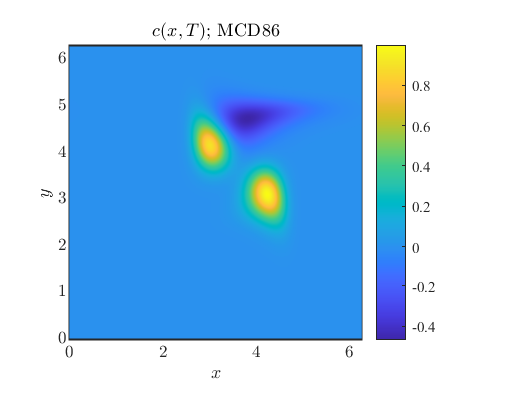
\includegraphics{figs/c_final_MCD86}
    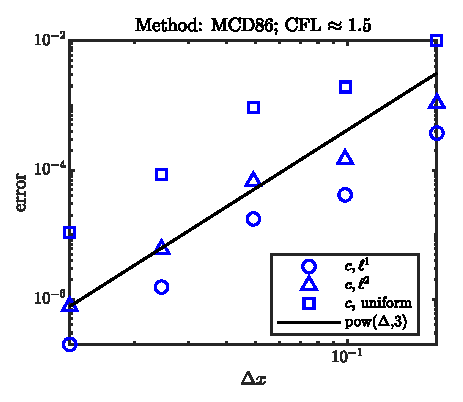
\includegraphics{figs/conv_order_MCD86}
    \caption{}\label{fig:c_final_MCD86}
\end{figure}

The last method reaches high order convergence but it uses an opaque cancellation of error. High order accuracy can be reach for the linear advection problem more easily by using readily available ODE solver on \eqref{eq:x_ODE}. For example, we could use RK4 method to reach 4th order accuracy. We have RK4 applied to \eqref{eq:x_ODE}:
\begin{align*}
    \ve x^1 &= \ve x_i;\quad &&\ve u^1 = \ve u(x^1,t^{n+1})\\
    \ve x^2 &= \ve x_i - \frac{\Delta t}{2} \ve u^1;\quad&&\ve u^2 = \ve u(x^2,t^{n+1/2})\\
    \ve x^3 &= \ve x_i - \frac{\Delta t}{2} \ve u^2;\quad&&\ve u^3 = \ve u(x^2,t^{n+1/2})\\
    \ve x^4 &= \ve x_i - \Delta t \ve u^3;\quad&&\ve u^4 = \ve u(x^4,t^{n})\\
\end{align*}
then
\begin{align*}
    \ve u^s = (\ve u^1+2\ve u^2+2\ve u^3+\ve u^4)/6.
\end{align*}
and 
\begin{align*}
    c(\ve x_i,t^{n+1}) = c(\ve x_i-\ve u^s\Delta t,t^{n}).
\end{align*}
Now that the departure point is solve to fifth order locally, we need a fifth order interpolation as well. We instead just use FINUFFT which is spectral. For all other interpolations within the RK4 steps, we could use one less order, thus \texttt{spline} is used. Fig. \ref{fig:c_final_RK4SL} shows good convergence result. 
\begin{figure}[H]
    \centering
    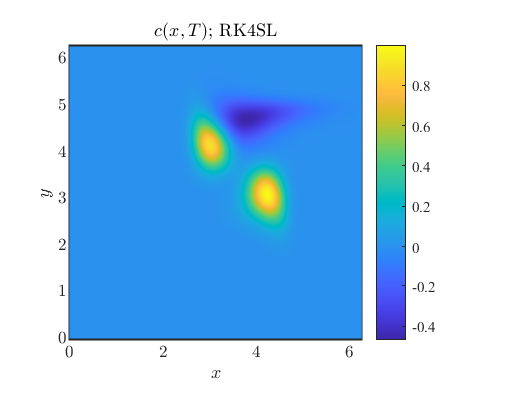
\includegraphics{figs/c_final_RK4SL}
    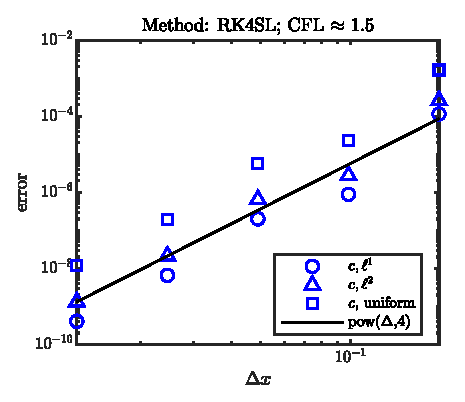
\includegraphics{figs/conv_order_RK4SL}
    \caption{}\label{fig:c_final_RK4SL}
\end{figure}
It is curious why \sml\ method literature does not use RK method to solve for the departure point. We check the cost by counting the number of interpolations and their requires order. We compare RK3, which should be third order, with MCD86: RK3 needs three third and a forth order interpolation, while MCD86 needs two second, two third, and two forth order interpolation. It seems MCD86 is more expensive. We comment that the second and third RK4 step looks like a fixed point solver, and it might be that the RK4 method and classic \sml\ methods are more similar than the form suggests. We will continue the discussion in Section \ref{sec:nonli_adv} where the issue is a bit more nuanced. 

We could replace all the interpolation with FINUFFT so that they are spectrally accurate. We give a large enough $Nx = Ny$ so that there is no spatial error (for 3 Gaussian, $Nx = Ny = 81$). Then we can fix the spatial resolution and improve accuracy by only refining the timestep. This is a good way to isolate the error produced by the timestepping. But this is also viable numerical method. In a sense, the method is pseudospectral but with with \sml\ timestepping. This has real advantage compared to the regular pseudospectral method for advection in that it could take a lot bigger a timestep while still being stable. For example, to solve the problem above, \sml\ Pseudospectral method is stable for CFL number up to 3 while the regular IF-RK4 Pseudospectral method is only stable when CFL number is less than 0.5. Fig. \ref{fig:conv_order_finu_} shows the convergence order result for \sml\ Pseudospectral and IF-RK4 Pseudospectral method. We see that all the convergence order of \sml\ method stay the same. In particular, the error for the most accurate result for RK4SL Pseudospectral method is $O(10^{-9})$, very small! And that is achieved with 54 timestep (i.e.: $\Delta t = 0.0093$). IF-RK4 Pseudospectral method does not each the same level of accuracy with same number of timestep (the $x$-axis of the IF-RK4 figure is large than the rest). To truly compare the two methods, we also need to know the cost per timestep. Assuming that FINUFFT cost as much as a standard uniform Fast Fourier Transform (FFT), we approximate the cost by counting the number of \texttt{fft/ifft} pairs per timestep. For IF-RK4, assume that the velocity is given in Fourier space and we solve for the tracer in Fourier space, we only need four pairs of \texttt{fft/ifft} per timestep. The \sml RK4  Pseudospectral method needs four $u,v$ interpolation and one tracer field interpolation, and that is $4\times 2+1 = 9$ \texttt{fft/ifft} pairs. Therefore we could say \sml RK4 w/ FINUFFT is as expensive as two IF-RK4 method. But compare the stability and accuracy of the two methods shown in Fig. \ref{fig:conv_order_finu_}, we see that IF-RK4 needs more than two times the timestep to reach the same accuracy. Therefore we conclude that \sml RK4 w/ FINUFFT is cheaper as a solver for linear advection.
\begin{figure}[H]
    \centering
    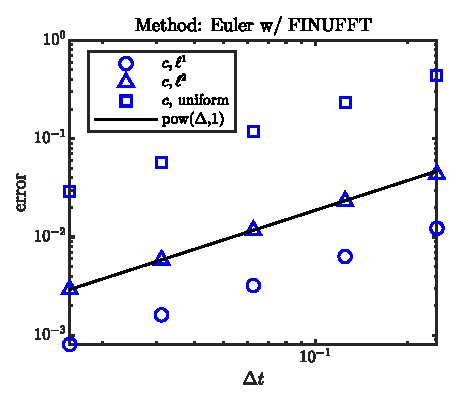
\includegraphics{figs/conv_order_finu_Euler}
    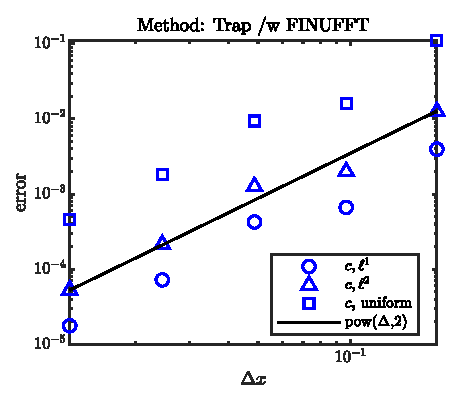
\includegraphics{figs/conv_order_finu_Trap}
    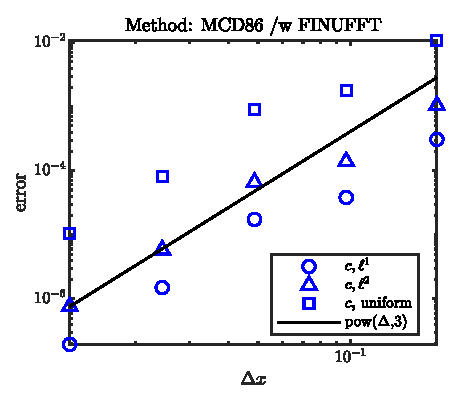
\includegraphics{figs/conv_order_finu_MCD86}
    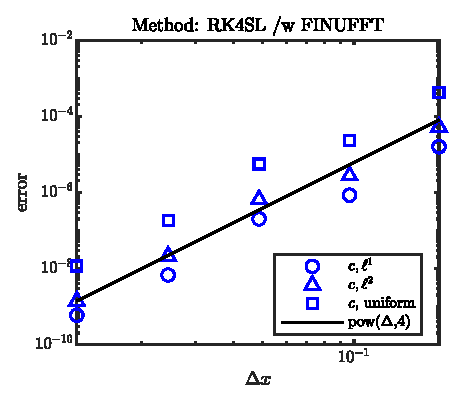
\includegraphics{figs/conv_order_finu_RK4SL}
    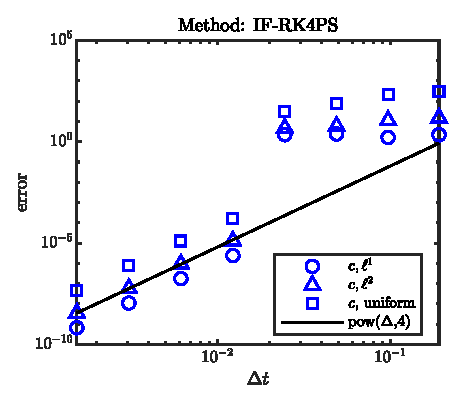
\includegraphics{figs/conv_order_finu_IFRK4}
    \caption{}\label{fig:conv_order_finu_}
\end{figure}

\section{Semi-Lagrangian Method for 2D Navier Stokes}\label{sec:nonli_adv}
We use \sml\ methods to numerically solve the incompressible inviscid Navier-Stokes equation:
\begin{align}
    \begin{cases}
    \pe_t\ve u+\ve u\cdot\nabla\ve u=-\nabla p\\
    \nabla\cdot\ve u = 0.
    \end{cases}\label{eq:2d_Nav}
\end{align}
This is possible because we could reformulate the equation in the vorticity-stream formulation, which is an advection equation with vorticity as the tracer. First, due to incompressibility, we could define the streamfunction $\psi$ and the vorticity $\omega$ ($u$ is the $x$-component of $\ve u$ and $v$ is the $y$-component of $\ve u$):
\begin{align}
    &-\pe_y \psi = u,\quad  \pe_x \psi = v;\nonumber\\
    &\omega = -\pe_y u+\pe_x v = \nabla^2 \psi.\label{eq:relate_omega_psi}
\end{align}
Then the vorticity-stream formulation is:
\begin{align}
    &\pe_t\omega+\ve u\cdot\nabla\omega = 0\label{eq:vort_stream}\\
    \fff&\pe_t\omega+J(\psi,\omega) = 0\nonumber
\end{align}
and this equation is closed since $\ve u,\psi$ can be solved from $\omega$ via \eqref{eq:relate_omega_psi}. This is a nonlinear advection problem since the velocity that advect tracer field needs to solved from the tracer field $\omega$. Therefore for each timestep we only know the velocity information at time $t^n$. 

To test our \sml\ schemes, we use them to solve the D Navier-Stokes problem with two different initial condition. First, we initialize the $\omega$ field to be the one associated with the Taylor vortex \eqref{eq:taylor}. We use $L = 1$ and $v_0 = 1$ and solve till time $T = 0.25$. To obtain the error of the solver, we compare the error with the truth $\omega$ given by the formula. The second initial condition is the three Gaussian (now three vortices) given by \eqref{eq:3Gauss}. For this we use $L = 2\pi$ and $v_0 = 1$ and solve till time $T = 1.5$. We estimate the error empirically for this case. 

Now we show the result for the \sml\ schemes. Fig. \ref{fig:nonlin_conv_order_Taylor_Euler} shows the result for Euler timestepping. For Euler, only velocity information at $t^n$ is needed and no change is needed from our previous description of the method. The first row are results for the Taylor initial condition while the second row is for the three vortices initialization. Left column is the classic \sml\ methods where we refine space and time together while keeping the CFL number about 1.5. The right column we use FINUFFT for the interpolation, thus we keep the space resolution constant ($Nx = Ny = 9$ for Taylor and $Nx = Ny = 33$ for three vortices) and refine only time. All four plots shows the expected first order convergence. 
\begin{figure}[H]
    \centering
    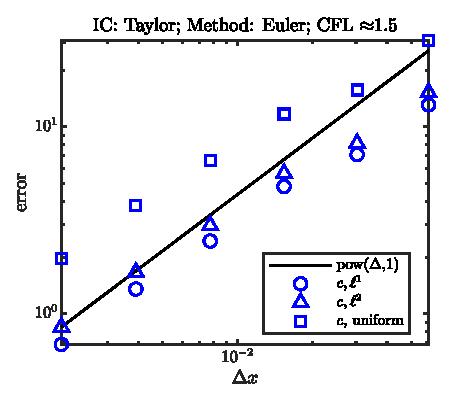
\includegraphics{figs/nonlin_conv_order_Taylor_Euler}
    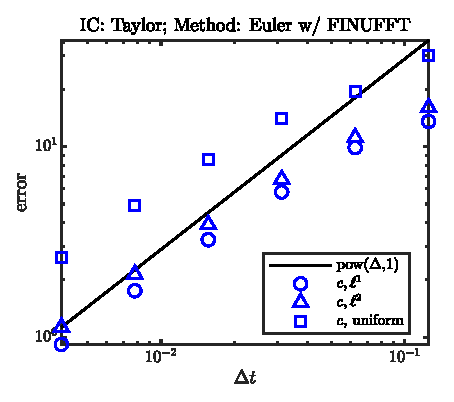
\includegraphics{figs/nonlin_conv_order_Taylor_finu_Euler}
    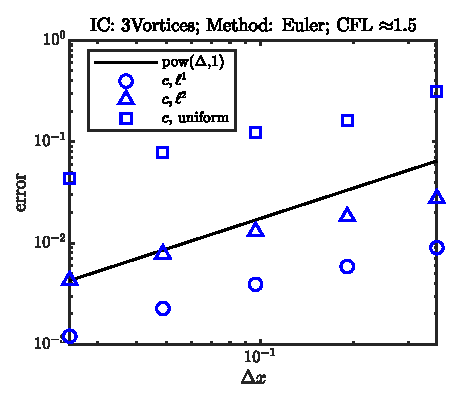
\includegraphics{figs/nonlin_conv_order_3Vortices_Euler}
    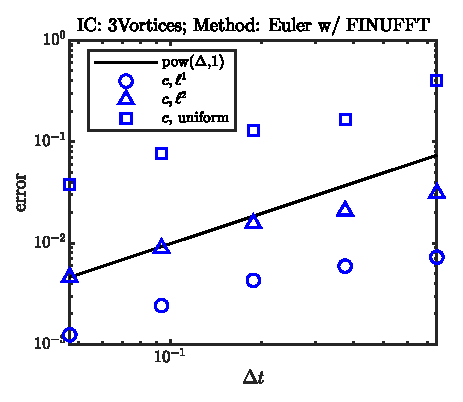
\includegraphics{figs/nonlin_conv_order_3Vortices_finu_Euler}
    \caption{}\label{fig:nonlin_conv_order_Taylor_Euler}
\end{figure}

Now for the trapezoidal method, we need an estimate of the velocity at $t^{n+1}$. To do this we extrapolate it from the velocity at $t^n$ and $t^{n-1}$ via
\begin{align*}
    \ve u(t^{n+1}) = 2\ve u(t^n)-\ve u(t^{n-1}). 
\end{align*}
Then we have $\ve u$ available on the grid at time $t^{n+1}$. But now we need the information for the velocity at $t^{n-1}$, so for the first step, we call the Euler method instead. Now we can proceed as we have stated in Section \ref{sec:linear_adv}. Fig. \ref{fig:nonlin_conv_order_Taylor_Trap} shows convincing second order convergence. 
\begin{figure}[H]
    \centering
    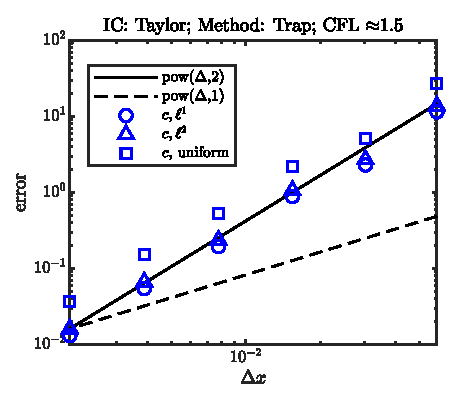
\includegraphics{figs/nonlin_conv_order_Taylor_Trap}
    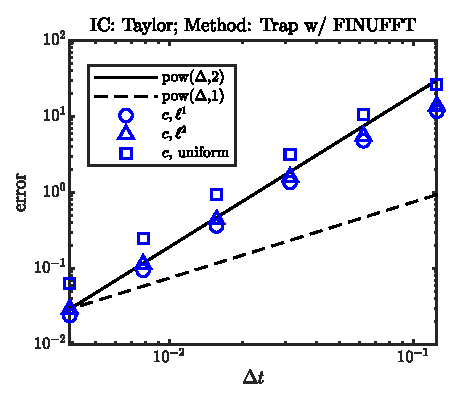
\includegraphics{figs/nonlin_conv_order_Taylor_finu_Trap}
    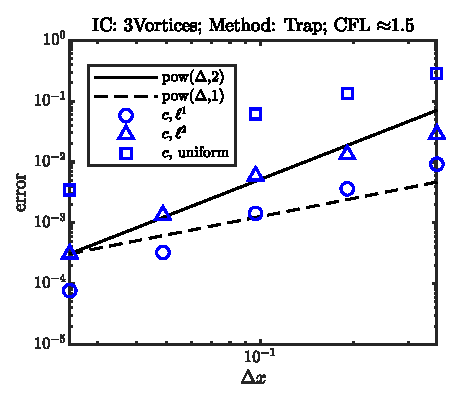
\includegraphics{figs/nonlin_conv_order_3Vortices_Trap}
    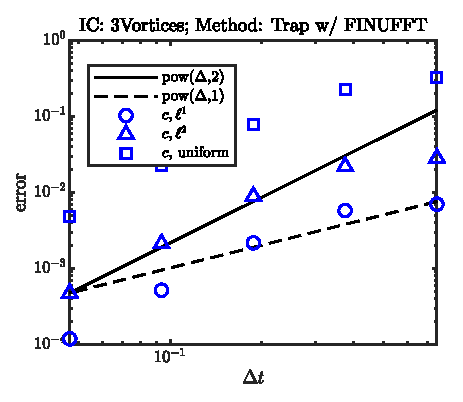
\includegraphics{figs/nonlin_conv_order_3Vortices_finu_Trap}
    \caption{}\label{fig:nonlin_conv_order_Taylor_Trap}
\end{figure}
The MCD86 method need the estimate of the velocity at the half timestep $t^{n+1/2}$. Since we want global third order accuracy, the order of the extrapolation needs to be improved as well compared to one used in the trapezoidal method. For this \cite[(19)]{mcdonald1987} uses an extrapolation stated in \cite{temperton1987}, but this is just the standard polynomial extrapolation
\begin{align*}
    \ve u(t^{n+1/2}) = \frac{1}{8}\left(15\ve u(t^n)-10\ve u(t^{n-1})+3\ve u(t^{n-2})\right). 
\end{align*}
For the first two steps where we do not have the velocity information at $t^{n-1}$ and $t^{n-2}$, we call the trapezoidal method. With this estimate, we could proceed with the method as stated in Section \ref{sec:linear_adv}. Fig. \ref{fig:nonlin_conv_order_Taylor_MCD86} shows good third order convergence result.
\begin{figure}[H]
    \centering
    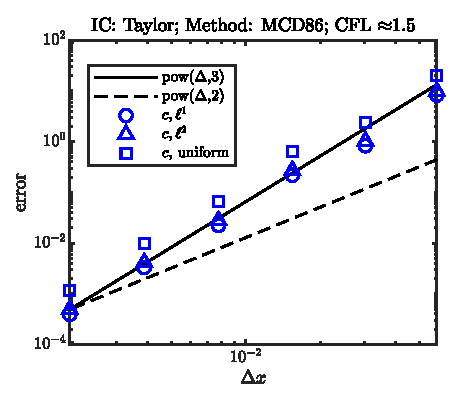
\includegraphics{figs/nonlin_conv_order_Taylor_MCD86}
    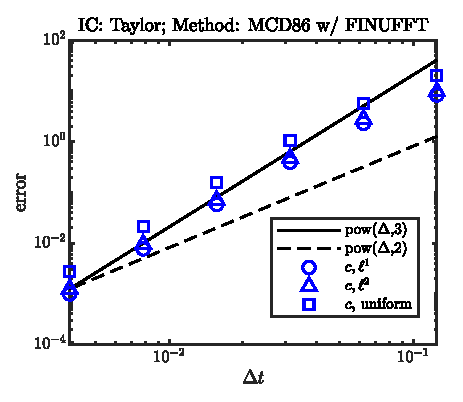
\includegraphics{figs/nonlin_conv_order_Taylor_finu_MCD86}
    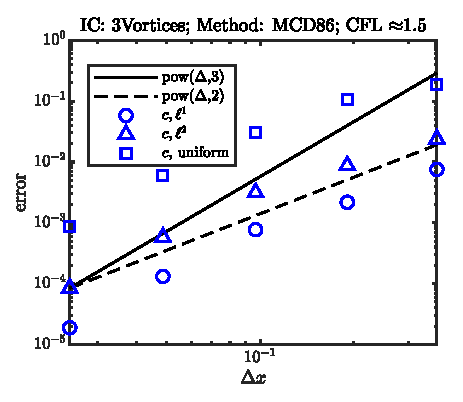
\includegraphics{figs/nonlin_conv_order_3Vortices_MCD86}
    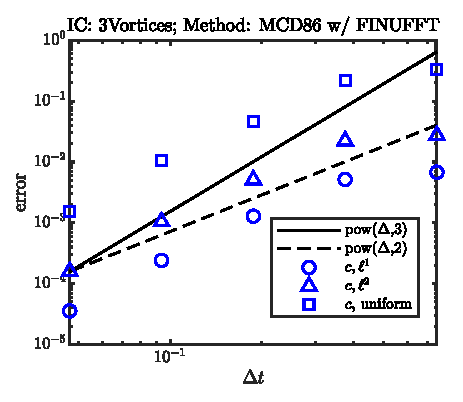
\includegraphics{figs/nonlin_conv_order_3Vortices_finu_MCD86}
    \caption{}\label{fig:nonlin_conv_order_Taylor_MCD86}
\end{figure}
The story for RK4 method is less straightforward. We could not reach fourth order convergence. This is because a fourth order extrapolation using the information at $t^n$ to $t^{n-3}$ does not appear to be stable, in the sense that with that extrapolation for $\ve u(t^{n+1/2}),\ve u(t^{n+1})$, the solution does not converge. So instead we use the same third order extrapolation as the one used in MCD86 method:
\begin{align*}
    \ve u(t^{n+1/2}) &= \frac{1}{8}\left(15\ve u(t^n)-10\ve u(t^{n-1})+3\ve u(t^{n-2})\right);\\
    \ve u(t^{n+1}) &= 3\ve u(t^n)-3\ve u(t^{n-1})+\ve u(t^{n-2}).
\end{align*}
Initialize the first few steps with MCD86, we can proceed with the description of RK4 from Section \ref{sec:linear_adv}. But the result is only third order as shown in Fig. \ref{fig:nonlin_conv_order_Taylor_RK4SL}.
\begin{figure}[H]
    \centering
    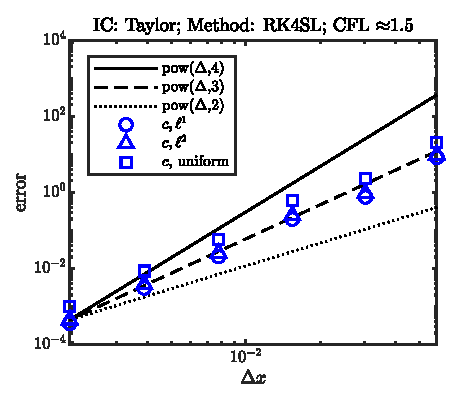
\includegraphics{figs/nonlin_conv_order_Taylor_RK4SL}
    \includegraphics{figs/nonlin_conv_order_Taylor_finu_RK4SL}
    \includegraphics{figs/nonlin_conv_order_3Vortices_RK4SL}
    \includegraphics{figs/nonlin_conv_order_3Vortices_finu_RK4SL}
    \caption{}\label{fig:nonlin_conv_order_Taylor_RK4SL}
\end{figure}
We continue the discussion of using RK method in \sml setting. The above result is an discouragement, but we still argue that RK3 is an strong alternative to MCD86. Only needing third order extrapolation, RK3 could reach third order convergence as RK4 above. And we have determined that RK3 is cheaper then MCD86 per timestep.

In general, for nonlinear advection problem, extrapolation to get an estimate of the velocity field seems sketchy to me even when it seems that it works for low order extrapolation with moderate timestep (but still CFL number larger than one). And it is not a good idea to push the order higher, as shown in the RK4 example. I am interested in if there is an alternative high (larger than three) order \sml\ method that does not use polynomial extrapolation. 

\section{Semi-Lagrangian Method for 2D Linear Advection, Cont.}\label{sec:adv_NS}
We finish the note by solving linear advection problems where the velocity is obtained numerically. Given the disappointing result of \sml\ method when applied to nonlinear advection, we choose to stick with IF-RK4 method to solve the velocity. But for advection of the tracer, we use \sml RK4 w/ FINUFFT to solve. This work well with the pseudospectral IF-RK4 since we can keep space resolution fixed while improve the accuracy by refining time. Since the \sml\ allows for larger timestep then IF-RK4, we use four steps of IF-RK4 to solve velocity within each single step of tracer solve using \sml\ RK4 w/ FINUFFT. Note here that we record the velocity at middle time $t^{n+1/2}$ and end time $t^{n+1}$ for use in the tracer solve.

First we solve the problem we solve in Section \ref{sec:linear_adv} but now with the velocity numerically solved. We initialize the $\omega$ field with the Taylor vortices \eqref{eq:taylor} and the tracer field as three Gaussians \eqref{eq:3Gauss}. We again have $L = 2\pi, v_0 = 1$, and we solve still $T = 0.5$. We fix $Nx = 81$ and refine $Nt = 2:32$. We same the data from a high fidelity (estimated error less than $10^{-14}$) result from the IF-RK4 method in Section \ref{sec:linear_adv} as the ``truth'' to calculate the error. Fig. \ref{fig:NSAdv_c_final_Taylor_3Gaussian} left shows the final tracer field for the solute with the finest time resolution, and the right shows the convergence result. We see that the final tracer field is similar to the ones we have seen in Section \ref{sec:linear_adv}, this is reassuring. And we see fourth order convergence once the timestep is small enough for the IF-RK4 velocity solver. We note here that a fourth order \sml\ nonlinear advection solver should remove this barrier. 
\begin{figure}[H]
    \centering
    \includegraphics{figs/NSAdv_c_final_Taylor_3Gaussian}
    \includegraphics{figs/NSAdv_conv_order_Taylor_3Gaussian}
    \caption{}\label{fig:NSAdv_c_final_Taylor_3Gaussian}
\end{figure}

Now we solve the problem where the velocity is initialize with three vorticity \eqref{eq:3Gauss}, and the tracer has initial condition sinp \eqref{eq:sinp2}. 
\begin{figure}[H]
    \centering
    \includegraphics{figs/NSAdv_c_final_3Vortices_sinp}
    \includegraphics{figs/NSAdv_conv_order_3Vortices_sinp}
    \caption{}\label{fig:NSAdv_c_final_3Vortices_sinp}
\end{figure}

\newpage
\bibliographystyle{alpha}
\bibliography{citation}

\end{document}









